\chapter{Konzepte von Predictive Analytics}
\label{part:Konzepte_PA}

\section{Begriffsdefinition}

Das primäre Ziel von Predictive Analytics ist das Treffen von
Vorhersagen.
Hierbei sind nicht nur Prognosen für die Zukunft gemeint, sondern
auch Einschätzungen und Beurteilungen unklarer Situationen, bei denen die für
die Entscheidungsfindung wichtigen Daten fehlen (vgl. \cite{Dinov}, S.~9~f.).
Hier sind einige Anwendungsbeispiele, die verdeutlichen, wie Predictive
Analytics eingesetzt werden kann (vgl. \cite{Schmitz}):

\begin{description}

\item[Betrugserkennung (\emph{fraud detection}):] \hfill \\
Geschäftsvorgänge werden automatisch analysiert, in der Hoffnung, dass
Unregelmäßigkeiten vom System erkannt werden. Verdächtige Vorgänge können dann
zum Beispiel einer manuellen Prüfung unterzogen werden.

\item[Vorhersage von Wartungszeitpunkten (\emph{predictive
  maintenance}):] \hfill \\
Automatische Systeme schätzen die Ausfallwahrscheinlichkeit von Maschinen ein
und bestimmen den Zeitpunkt für die nächste Inspektion.

\item[Verringerung von Ausschuss (\emph{predictive quality}):] \hfill \\
Mit Hilfe von Sensordaten werden fehlerhafte Produkte im Produktionsprozess
erkannt und aussortiert.

\item[Erkennung von Kundenunzufriedenheit (\emph{churn management}):] \hfill \\
Muster in Daten, die auf Unzufriedenheit von Kunden deuten, automatisch erkennen
und rechtzeitig Gegenmaßnahmen versuchen.

\item[Verbesserung der Zahlungsmoral:] \hfill \\
Mit Hilfe von Vorhersagen die Randbedingungen verbessern, sodass Kunden
schneller Rechnungen begleichen.

\item[Bessere Kontrolle von Personalfluktuationen:] \hfill \\
Mitarbeiter, die bald einen Arbeitsplatzwechsel vollziehen könnten, mit Hilfe
von Vorhersagemodellen erkennen, um rechtzeitig darauf reagieren zu können.

\end{description}

\begin{figure}%[!hbt]
\centering
\caption{Erstellung von Vorhersagemodellen.}
\includegraphics[scale=0.8]{Grafiken/PA_Ink.pdf} 
\label{pic:PA}
\end{figure}
Abbildung~\ref{pic:PA} veranschaulicht den allgemeinen Prozess zur Generierung
von Vorhersagemodellen\footnote{
Basierend auf dem Original aus \cite{Parthasarathy}.
}.
Zum Erstellen der Vorhersagen werden historische Daten benötigt. Diese Daten
werden von Algorithmen genutzt, um Modelle zu bauen. Die Vorhesagemodelle
akzeptieren neue Daten als Eingabe und liefern dazu eine Vorhesage der
gewünschten Eigenschaften. So könnte eine Versicherung beispielsweise
Vorhersagemodelle zur Betrugserkennung implementieren. Die historischen Daten
könnten in diesem Fall Forderungen von Kunden an die Versicherung aus der
Vergangenheit sein. Das Vorhesagemodell würde dann eine neue Forderung an die
Versicherung als Eingabe nehmen und könnte als Ausgabe eine Zahl zwischen 0 und
1 liefern. Dieser vorhergesagte Wert kann dann als Wahrscheinlichkeit
interpretiert werden, dass es sich bei der neuen Forderung um einen Betrugsfall
handelt. 

Weiterhin wird zwischen Descriptive, Predictive und Prescriptive Analytics
unterschieden (vgl. \cite{Martin}):

\begin{description}

\item[Descriptive Analytics:] \hfill \\
Damit wird der Prozess der Beschreibung von Daten bezeichnet. Dies soll ein
Verständnis für die Daten und ihre Zusammenhänge liefern.
Descriptive Analytics kann als eigenständiger Prozess durchgeführt werden, oder
als Vorstufe für weitere Analysen dienen.

\item[Predictive Analytics:] \hfill \\
Predictive Analytics liefert Prognosen auf der Basis historischer Daten. Bei der
Unterscheidung zwischen den drei Analytics Varianten wird insbesondere der
zweite Schritt in Abbildung~\ref{pic:PA} betont, wenn von Predictive Analytics
gesprochen wird.

\item[Prescriptive Analytics:] \hfill \\
Prescriptive Analytics geht einen Schritt weiter als Predictive Analytics, indem
es, zusätzlich zur Prognose, Erklärungen abgibt, warum diese Prognose gemacht wurde.
Basierend darauf kann Prescriptive Analytics auch Handlungsempfehlungen liefern.

\end{description}

\section{Begriffsabgrenzung}

Unter Data Mining versteht man das Nutzen von statistischen Methoden zur
Analyse großer Datenmengen mit dem Ziel, neue Erkenntnisse zum untersuchten 
Thema oder Objekt zu erlangen\footnote{
Der Begriff Data mining ist also nicht wörtlich zu verstehen. Gemeint ist
nicht die Gewinnung von Daten, sondern die Gewinnung von Erkenntnissen aus den
Daten.
}
(vgl. \cite{McCarthy}, S.~6). Es bestehen große Schnittmengen mit
Predictive Analytics, insbesondere im Hinblick auf die Nutzung der
gleichen Methoden und Werkzeuge. Allerdings steht bei Data Mining nicht
explizit die Erstellung von Vorhersagen im Vordergrund.

Data Science kann als interdisziplinäres Feld verstanden werden, das mit
großen und komplexen Datenbeständen arbeitet. Das Ziel von Data Science
ist die Entwicklung von Algorithmen und Werkzeugen, die in der Lage sind, diese
Datenbestände zu nutzen, um Systeme zur Entscheidungsunterstützung zu
implementieren (\emph{semiautomated decision support systems}) (vgl.
\cite{Dinov}, S.~9).  Im Gegensatz zu Predictive Analytics steht bei 
Data Science eher die Entwicklung von Algorithmen im Vordergrund. 
Bei Predictive Analytics hingegen steht die Anwendung dieser Methoden im 
Fokus.

Ein im Zusammenhang mit Datenanalysen oft verwendeter Begriff ist Big Data.
Bei Big Data werden die großen Dimensionen der analysierten Daten betont, wobei
drei charakteristische Eigenschaften im Vordergrund stehen, nämlich Volume, Velocity 
und Variety (als \emph{3 Vs} abgekürzt; vgl. \cite{McCarthy}, S.~7-8). Dabei bezeichnet Volume
besonders große Mengen an Daten, Velocity die hohe Geschwindigkeit der Datenverarbeitung
und Variety die große Vielfalt der Datenquellen.

Business Analytics wird als Oberbegriff für Prozesse definiert, die
Analysemodelle im geschäftlichen Kontext erstellen (vgl. \cite{McCarthy}, S.~6)). 
Predictive Analytics und Data Mining werden dann als Bestandteil von Business Analytics
gesehen. 

Business Intelligence ist ein zu Business Analytics ähnlicher
Begriff und steht allgemein für Anwendungen und Techniken, die im
Geschäftsumfeld zur Entscheidungsunterstützung und zur Generierung von
Einsichten genutzt werden\footnote{
Manche Autoren betrachten den Begriff \glqq{Intelligence}\grqq{} als Anspielung
auf die gängige, englische Bezeichung für Aufklärungs- und Nachrichtendienste,
wie beispielsweise die CIA.
} (vgl. \cite{Gluchowski}, S.~89-90). Damit kann Predictive Analytics,
ähnlich wie bei Business Analytics, als ein Bestandteil von 
Business Intelligence eingeordnet werden (vgl. \cite{Gluchowski}, S.~92). 

Ein weniger verbreiteter Begriff ist Forecasting,
die Erstellung von Prognosen durch menschliche Beobachter. Im nächsten Abschnitt
wird diese Form von Vorhersagen genauer beschrieben und anschließend mit
Predictive Analytics verglichen.  

\section{Probleme menschlicher Urteile} \label{Probs}

Die meisten Urteile und Prognosen werden von Menschen gefällt, ohne statistische
Modelle und Vorhersagealgorithmen zu nutzen. Grundsätzlich fällt jeder Mensch
Urteile, macht Vorhersagen und nutzt diese um Entscheidungen zu treffen. Aus
diesem Grund ist ein gutes Urteilsvermögen eine Eigenschaft, die eigentlich
universell gebraucht wird. Für die großen gesellschaftlichen Entscheidungen
versorgen Experten Wirtschaft, Politik und Öffentlichkeit mit Prognosen und
Einschätzungen. Dabei ist es üblich routinemäßig Expertenmeinungen einzuholen,
unüblich ist es allerdings, systematisch die Qualität dieser Urteile zu
überprüfen (vgl. \cite{Tetlock}, S.~1). Aus diesem Grund hat der Psychologe
Philip Tetlock sich zur Aufgabe gemacht, \glqq{gutes} Urteilsvermögen\grqq
formal fassbar zu machen (vgl. \cite{Tetlock}, S.~3). Nach Tetlock sollte gutes
Urteilsvermögen anhand zweier Kriterien gemessen werden (vgl. \cite{Tetlock},
S.~7):
\begin{description}
\item[(1) Richtigkeit der Vorhersagen (\emph{get it right}):] \hfill \\
\label{misc:Emp_Korr}
Empirische Korrespondenztests sollen genutzt werden, um zu überprüfen, wie gut
die Meinungen und Vorhersagen von Experten mit der Wirklichkeit übereinstimmen.
\item[(2) Logische Konsistenz des Denkmodells (\emph{think the right way}):] \hfill \\
Die Gedanken von Experten sollten logisch konsistent sein. Genauer ausgedrückt
bedeutet dies, dass die Denkmodelle nicht die Gesetze der Logik und der
Wahrscheinlichkeitstheorie missachten sollten. Zudem sollte eine Person mit
einem guten Urteilsvermögen ihre Glaubenssätze an neue Erkenntnisse anpassen
können.
\end{description}
Dabei sollte die experimentelle Psychologie die notwendigen Fakten und
Einsichten liefern (vgl. \cite{Tetlock}, S.~8).

\subsection{Tetlocks Forecasting Exercises}

Für die empirischen Korrespondenztests führten Tetlock und sein Team eine Reihe
von Forecasting Exercises mit Experten durch. Diese Expertenbefragungen
wurden bereits in Teil~\ref{part:Schw_Vorhersagen} thematisiert und sollen nun
detaillierter erläutert werden.

Insgesamt wurden die Urteile von 284 Experten analysiert. Diese hatten im
Durchschnitt 12 Jahre Berufserfahrung und die Hälfte (52~\%) besaß einen
Doktortitel. Etwa 61~\% der Teilnehmer wurden mindestens einmal von den Medien
interviewt und 21~\% mehr als zehnmal. Etwa 80~\% der Experten waren mindestens
einmal als Berater für internationale politische oder wirtschaftliche
Angelegenheiten tätig. (vgl. \cite{Tetlock}, S.~239-240)

Die Befragten sollten Prognosen erstellen, indem sie auf Fragen zu zukünftigen
Entwicklungen in Politik und Wirtschaft antworteten. Dabei handelte es sich um
feste Fragestellungen, die von den Forschern zuvor ausgewählt wurden. Zu den in
den Fragen formulierten Szenarien sollten die Befragten subjektive
Wahrscheinlichkeiten\footnote{
Eine subjektive Wahrscheinlichkeit wird als Grad des Vertrauens einer Person in
den Eintritt eines Ereignisses interpretiert (vgl. \cite{Eisenfuehr}, S.~152).}
angeben. (vgl. \cite{Tetlock}, S.~245)

Die Sammlung der Expertenprognosen begann 1987 und erstreckte sich über mehr als
zehn Jahre. Dabei wurden Fragen über die zukünftige Entwicklung von etwa 60
Nationen gestellt. (vgl. \cite{Tetlock}, S.~242)

Weiterhin wurden die Fragen in folgende Themenbereiche untergliedert
(vgl. \cite{Tetlock}, S.~246-248):
\begin{description}
\item[(a)] Kontinuität politischer Führung
\item[(b)] Innen- und Wirtschaftspolitik
\item[(c)] Nationale Sicherheit und Verteidigungspolitik
\item[(d)] Zusätzliche Spezialthemen
\end{description}
Insgesamt wurden 82 361 subjektive Wahrscheinlichkeiten eingeholt, die als
Antwort auf circa 27 450 Fragen gegeben wurden. (vgl. \cite{Tetlock}, S.~246)

\subsection{Der Brier Score als Maß der Genauigkeit von Vorhersagen}

Die Fragen der Forecasting Exercises wurden so formuliert, dass bei allen
nach einer gewissen Zeitspanne festgestellt werden konnte, ob und welches der
möglichen Szenarien\footnote{
Die möglichen Szenarien müssen dabei logisch vollständig sein und sich
gegenseitig ausschließen (\emph{logically exhaustive and mutually exclusive};
vgl. \cite{Tetlock}, S.~245).
} tatsächlich eingetreten ist. Um dann die, auf Seite~\pageref{misc:Emp_Korr}
erwähnte, Richtigkeit der Vorhersagen zu überprüfen, müssen die subjektiven
Wahrscheinlichkeiten mit der eingetretenen Wirklichkeit verglichen werden. 

Das Werkzeug zur Durchführung dieses Vergleichs und zur Bewertung der
Genauigkeit der erstellten Prognosen ist der Brier Score (vgl. \cite{Tetlock}, S.~46). Dabei werden die subjektiven
Wahrscheinlichkeiten (die Vorhersagen) mit den tatsächlich eingetretenen
Ereignissen (der Wirklichkeit) verrechnet\footnote{
  Es wird 0 eingesetzt, falls ein Szenario nicht eingetreten ist und 1 falls es
  eingetreten ist (vgl. \cite{Tetlock}, S.~46-47).
}. Das Ergebnis ist eine Zahl zwischen 0 und 1, wobei 0 die beste und 1 die
schlechteste Wertung darstellt. Wenn ein Prognostiker jedes Ereignis, das
schließlich eintritt, als unmöglich eingestuft hat und jedes Ereignis, welches
ausbleibt, als sicher, dann endet er beim schlechtesten Brier Score von 1. Die beste Wertung von 0 kann hingegen nur erreicht werden, indem
man, zumindest was die gestellten Fragen betrifft, hellseherische Fähigkeiten
beweist und jedes eingetretene Ereignis mit einer subjektiven Wahrscheinlichkeit
von 1 bewertet und jedem ausgebliebenen Ereignis eine 0 zugewiesen hat (vgl.
\cite{Tetlock}, S.~47).

Zudem lässt sich der Brier Score in zwei Komponenten zerlegen, die
von den Fähigkeiten des Prognostikers abhängen: Kalibrierung
(\emph{calibration}) und Diskriminierung (\emph{discrimination})\footnote{
  Die Bedeutung dieser beiden Komponenten wurde auch im einleitenden
  Teil~\ref{part:Schw_Vorhersagen} erläutert.
} (vgl. \cite{Tetlock}, S.~47). \\ \\
Die Kalibrierung misst wie gut ein Prognostiker
Ereignisse in Wahrscheinlichkeitskategorien einordnen kann\footnote{
  10~\% der Ereignisse aus der 0.1 Kategorie treten ein, 20~\% der Ereignisse
  aus der 0.2 Kategorie usw. 
}. Der Wertebereich der Kalibrierung liegt zwischen 0 und 1, wobei 0 den besten
und 1 den schlechtesten Wert darstellt (vgl. \cite{Tetlock}, S.~275). 

Die Diskriminierung misst wie gut sich die subjektiven Wahrscheinlichkeiten des 
Prognostikers von der relativen Häufigkeit (\emph{base-rate}) aller betrachteten
Ereignisse abheben. Der Wertebereich der Diskriminierung reicht von 0 bis zu
einem Wert, der die Unsicherheit der Umgebung, für die die Prognosen erstellt
werden, widerspiegelt (vgl. \cite{Tetlock}, S.~278). Im Falle der
Diskriminierung ist 0 der schlechteste Wert. Im besten Fall ist der Wert der
Diskriminierung gleich dem Wert der Unsicherheit. 

Die Kernidee bei der Anwendung des Brier Score ist das Nutzen
des Gesetzes der großen Zahlen (\emph{law of large numbers})
(vgl. \cite{Tetlock}, S.~12-13). Einzelne Urteile mit subjektiven
Wahrscheinlichkeiten, die nicht 0 oder 1 sind, können nicht widerlegt werden,
da seltene Ereignisse eintreten können und häufige Ereignisse ausbleiben können.
Betrachtet man hingegen eine große Zahl an Vorhersagen, dann kann mit Hilfe
des Brier Score die Genauigkeit des Prognostiker aus der Gesamtheit
seiner Vorhersagen eingeschätzt werden. 

Der Anhang~\ref{Anhang_Brier} liefert die Formeln für den Brier Score, wobei
dessen Berechnung zusätzlich anhand von Beispielen erläutert wird. 


\subsection{Detaillierte Ergebnisse der Forecasting Exercises}

Die Analyse der Ergebnisse der Forecasting Exercises konnte Aufschluss
darüber geben, welche Attribute der Teilnehmer einen Einfluss auf die
Genauigkeit ihrer Vorhersagen haben und welche nicht. 

Zu den Attributen, die \emph{keinen} Einfluss auf die Fähigkeiten der Experten
hatten, gehörten überraschenderweise (vgl. \cite{Tetlock}, S.~68):

\begin{description}

\item[(a) Bildungsgrad:] \hfill \\
Es gab keinen Zusammenhang zwischen Bildungsgrad und Genauigkeit der Vorhersagen.
Insbesondere spielte ein Doktortitel keine Rolle.

\item[(b) Fachgebiet:] \hfill \\
Es war kein Fachgebiet erkennbar, das den jeweiligen Experten in diesem Gebiet
einen Vorteil in Bezug auf die Genauigkeit der Prognosen gegenüber Spezialisten
aus anderen Gebieten bot.

\item[(c) Erfahrung:] \hfill \\
Es spielte keine Rolle, wie lange ein Experte in seinem Gebiet tätig war oder
wie oft er schon eine beratende Funktion übernommen hatte.

\item[(d) Zugang zu geheimen Informationen:] \hfill \\
Möglicherweise das überraschendste Ergebnis ist, die Tatsache, dass die Experten,
die einen Zugang zu vertraulichen Informationen hatten, keinen Vorteil gegenüber
anderen Teilnehmern in Bezug auf die Genauigkeit ihrer Prognosen hatten.

\end{description}
Zudem hat Medienberühmtheit einen starken negativen Effekt auf die Fähigkeiten
der Prognostiker (vgl. \cite{Tetlock}, S.~68). 

Ein entscheidender Faktor, der gute von schlechte Prognostikern unterscheidet,
ist nicht ihr Weltbild, sondern ihre Art zu Denken (\emph{cognitive style})
(vgl. \cite{Tetlock}, S.~72 und S.~75). Tetlock unterteilt die Experten in
Abhängigkeit von ihrer Art zu Denken in Füchse (\emph{foxes}) und Igel
(\emph{hedgehogs})\footnote{
In Anlehnung an das Essay \emph{The Hedgehog and the Fox} des Philosophen Isaiah
Berlin.
}. Genauer ausgedrückt, ist das wichtigste Maß für den Kognitive Style
eines Experten ein Wert auf einer kontinuierlichen Skala (vgl. \cite{Tetlock},
S.~87). An einem Ende der Skala befinden sich die Foxes, an dem anderen
die Hedgehogs. Dazwischen befinden sich die hybriden Ausprägungen
Fox-Hog (eher Fox als Hedgehog) und Hedge-Fox (eher
Hedgehog als Fox). Bestimmt wird der Wert als Ergebnis eines
Fragebogens (siehe \cite{Tetlock}, S.~241). Dabei ist der Punkt, der am
stärksten in die Gewichtung einfließt, die Frage nach der Selbstidentifikation
(vgl. \cite{Tetlock}, S.~74 Tabelle~3.3)\footnote{
Hierbei werden Gewichtungen angegeben, mit denen die einzelnen Fragen in
die Bewertung einfließen. Je höher der Betrag des Gewichts, desto stärkeren
Einfluss hat die Frage auf das Ergebnis. Das Vorzeichen des Gewichts gibt an,
in welche Richtung die jeweilige Frage das Ergebnis verschiebt. Ein negatives
Vorzeichen verschiebt den Wert auf der Skala in Hedgehog Richtung, ein
positives Vorzeichen hingegen in Fox Richtung.   
}. Diese Frage lautet übersetzt (siehe \cite{Tetlock}, S.~241):
\begin{quotation}
%\begin{spacing}{1.2}
Isaiah Berlin unterteilte Intellektuelle in Igel und Füchse. Der Igel kennt eine
große Sache und versucht so viel wie möglich innerhalb dieses konzeptionellen
Rahmens zu erklären, wohingegen der Fuchs viele kleine Dinge weiß und damit
zufrieden ist, von Fall zu Fall andere improvisierte Erklärungen zu
finden. Ich positioniere mich zum Igel- oder Fuchsende dieser Skala.
% Isaiah Berlin classified intellectuals as hedgehogs or
% foxes. The hedgehog knows one big thing and tries to explain as much as
% possible within that conceptual framework, whereas the fox knows
% many small things and is content to improvise explanations on a case-
% by-case basis. I place myself toward the hedgehog or fox end of this
% scale
%\end{spacing}
\end{quotation}
Abbildung~\ref{pic:Hedgehog_Fox} erläutert die Skala des Cognitive Style.

\begin{figure}%[!hbt]
\centering
\caption{Skala des Cognitive Style}%, mit den Charakterisierungen
%  \emph{Fox} und \emph{Hedgehog} als Gegenpole}
\includegraphics[scale=1]{Grafiken/Hedgehog_Fox.pdf} 
\label{pic:Hedgehog_Fox}
\end{figure}
Hedgehogs haben einige wenige Glaubenssätze, die sie nutzen um
Erklärungen für die unterschiedlichsten Dinge abzuleiten (vgl. \cite{Tetlock},
S.~73). Sie bemühen sich, Fakten in Einklang mit ihren präferierten Grundsätzen
zu bringen und fällen ihre Urteile, indem sie Schlussfolgerungen aus einer
kleinen Menge an Überzeugungen ziehen. Zudem tendieren Hedgehogs
zu intellektuellem \glqq{Geiz}\grqq (\emph{parsimony}) (vgl.\cite{Tetlock}, 
S.~20). Dies bedeutet, dass sie nur ungerne neue Grundsätze
aufstellen und stattdessen versuchen, mit ihren wenigen, schon vorhandenen
Glaubenssätzen weitreichende Erklärungen für eine große Bandbreite an Phänomenen
zu erhalten. Zudem zeichnen sich Hedgehogs durch eine starke
Selbstsicherheit in Bezug auf die Genauigkeit ihrer Prognosen und Urteile aus
(vgl. \cite{Tetlock}, S.~73). 

Foxes hingegen sind skeptisch bezüglich starker Glaubenssätze, die alles
umspannende Erklärungen liefern sollen. Stattdessen vertrauen sie auf viele
Grundsätze mit begrenzter Aussagekraft (\emph{tricks of their trade}) (vgl.
\cite{Tetlock}, S.~73). Weiterhin ist die Urteilsfindung bei Foxes keine
reine Übung in deduktiver Logik (vgl. \cite{Tetlock}, S.~73), sondern benötigt
die Integration diverser Informationsquellen. Foxes sind eher zaghaft,
wenn es darum geht, ihre eigenen Fähigkeiten als Prognostiker zu loben (vgl.
\cite{Tetlock}, S.~73-74). 

\begin{figure}%[!hbt]
\centering
\caption{Leistungsunterschiede bei den Forecasting Exercises in
  Abhängigkeit vom Cognitive Style der Teilnehmer}
\includegraphics[scale=0.88]{Grafiken/Tetlock_2_Ink.pdf} 
\label{pic:Tetlock_2}
\end{figure}

Ein Ergebnis von Tetlocks Forecasting Exercises wurde bereits in
Abbildung~\ref{pic:Tetlock_1} aus Teil~\ref{part:Schw_Vorhersagen} erläutert.
Dort war ersichtlich, dass die Experten im Vergleich zu statistischen
Algorithmen schlecht abschnitten. 

Abbildung~\ref{pic:Tetlock_2} zeigt nun ein differenzierteres Bild von der
Leistung der Experten\footnote{
Graphik basierend auf dem Original aus \cite{Tetlock} auf S.~77.
}. Abgebildet wird die Streuung der Leistung der Prognostiker in Abhängigkeit
von ihrem jeweiligen Cognitive Style\footnote{
Wie in Abbildung~\ref{pic:Hedgehog_Fox} wird eine Unterscheidung zwischen
Foxes}, Fox-Hogs, Hedge-Foxes und Hedgehogs gemacht.
Abbildung~\ref{pic:Tetlock_2} ist analog zu Abbildung~\ref{pic:Tetlock_1}.
Insbesondere sind wieder Kalibrierung und Diskriminierung\footnote{
Kalibrierung und Diskriminierung messen die Qualität der Vorhersagen eines
menschlichen Prognostikers oder eines (statistischen) Prognosemodells
(siehe S.~\ref{Kal_Dis}). Kalibrierung beschreibt die Fähigkeit eines
Prognostikers Ereignisse in richtige Wahrscheinlichkeitskategorien einzuordnen
(10\%-Ereignisse treten in 10~\% der Fälle ein, 20\%-Ereignisse in 20~\% der
Fälle usw.). Hohe Diskriminierung hingegen wird erreicht, wenn der Prognostiker
die Auftrittswahrscheinlichkeit einzelner Ereignisse von der Basisrate (
\emph{base rate}) aller Ereignisse unterscheiden kann. 
} in derselben Weise auf den Achsen abgebildet. Je weiter rechts-oben die
Wertung eines Prognostikers liegt, desto besser hat er bei den
Forecasting Exercises abgeschnitten.

In Abbildung~\ref{pic:Tetlock_2} wird deutlich, dass die Urteilskraft der
Expertengruppen im Hinblick auf Kalibrierung und Diskriminierung variiert. Die
Hedgehogs erzielen die schlechtesten Wertungen unter den Experten,
während Foxes und Fox-Hogs die besten Wertungen erhalten.
Insbesondere sind Foxes den Hedgehogs sowohl bezüglich der
Kalibrierungs- als auch bezüglich der Diskriminierungswertung überlegen.

Die statistischen Algorithmen waren allerdings besser als Foxes und
Hedgehogs. Die besten Foxes erhielten ähnliche Wertungen wie
Extrapolationsalgorithmen. Hedgehogs machten hingegen so große Fehler,
dass ihre Wertungen in der Nähe des zufallsbasierten Algorithmus liegen
\footnote{
Tetlock gebraucht als Umschreibung für den zufallsbasierten Algorithmus die
Metapher des \glqq{Dart spielenden Schimpansen}\grqq
(\emph{dart-throwing chimp}).
}. Insgesamt konnte keiner der Experten, weder Foxes noch
Hedgehogs auch nur annähernd in die Nähe der Wertung kommen, die vom
autoregressiven Modell\footnote{
Als Stufe 3 Algorithmus in Abbildung~\ref{pic:Tetlock_1} und als formales
Modell in Abbildung~\ref{pic:Tetlock_2} bezeichnet.
} erreicht wurde. (vgl. \cite{Tetlock}, S.~118)

 
\subsection{Gründe für die schlechte Leistung der Experten}

Auf Seite~\pageref{misc:Emp_Korr} wurden die Kriterien vorgestellt, nach denen
Forecaster, Tetlocks Meinung folgend, bewertet werden müssen:

\begin{description}

\item[(1) Richtigkeit der Vorhersagen] \hfill \\
Empirische Korrespondenztests werden beispielsweise mit Hilfe des Brier Scores
durchgeführt.

\item[(2) Logische Konsistenz des Denkmodells] \hfill \\
Die Denkmodelle der Forecaster sollten konsistent mit den Gesetzen der Logik
und Wahrscheinlichkeitstheorie sein.

\end{description}

Grundsätzlich ist Tetlock der Auffassung, dass die Experten bei den empirischen
Korrespondenztests (1) schlecht abgeschnitten haben, weil ihre Denkmodelle
nicht den Anforderungen der Gesetze der Logik und Wahrscheinlichkeitsrechnung 
(2) gerecht wurden (vgl. \cite{Tetlock}, S.~121). Hierbei identifiziert Tetlock
vier Prinzipien aus der Wahrscheinlichkeitstheorie, die befolgt werden müssen,
um ein gutes Urteilsvermögen zu erlangen\footnote{
Weitere Prinzipien, die identifiziert werden können, wären die logische und
zeitliche Konsistenz des Gedankenmodells einer Person. Die logische Konsistenz
kann erreicht werden, wenn die Glaubenssätze (Axiome) und Schlussfolgerungen,
die eine Person zur Urteilsfindung nutzt, frei von formal logischen
Widersprüchen sind. Die zeitliche Konsistenz ist gegeben, wenn die Person keinen
Geschichtsrevisionismus betreibt, also nicht versucht, ihre  (falschen bzw.
fehlerhaften) Urteile und Axiome nachträglich mit neuen Erkenntnissen zu
versöhnen.

Solche Regeln sollten prinzipiell auch beachtet werden, allerdings sind sie
auch weiter verbreitet und werden aus diesen Gründen hier nicht so ausführlich
behandelt.
} (vgl. \cite{Tetlock}, S.~301-302):

\begin{description}
\item[(1) Additive Regel (\emph{additive rule}):] \hfill \\
Die Wahrscheinlichkeit, dass mindestens eins von zwei sich gegenseitig
ausschließenden Ereignissen eintritt, ist die Summe der einzelnen
Wahrscheinlichkeiten.

\item[(2) Multiplikative Regel (\emph{multiplicative rule}):] \hfill \\
Die Wahrscheinlichkeit, dass zwei unabhängige Ereignisse eintreten, ist das
Produkt der Einzelwahrscheinlichkeiten.

\item[(3) Würdigung rivalisierender Weltsichten:] \hfill \\
Bei zwei konkurrierenden Weltsichten (Hypothesen)\footnote{
Die Weltsichten  müssen vollständig sein und sich gegenseitig
ausschließen
} sollten beide Ansichten in die Berechnung der Wahrscheinlichkeit für den
Eintritt eines Ereignisses fließen. Eine Hypothese braucht nur dann nicht
beachtet werden, wenn man sicher ist, dass ihr Wahrheitsgehalt bei 0 liegt.

\item[(4) Glaubensanpassung (\emph{belief updating}):] \hfill \\
Bei Eintritt eines Ereignisses sollte der Wahrheitsgehalt einer Weltsicht
angepasst werden, und zwar je nachdem, ob die betrachtete Weltsicht den Eintritt
dieses Ereignisses vorhergesagt hat oder nicht.

\end{description}

Die Regeln (3) und (4) basieren auf den Rechenregeln für bedingte
Wahrscheinlichkeiten und insbesondere auf der Formel von Bayes. Ausführlichere
Erläuterungen zu den vier Prinzipien der logischen Konsistenz befinden sich in
Anhang~\ref{Anhang_Bayes}. Dort werden die relevanten Formeln vorgestellt und es werden
einige Beispiele präsentiert.

Tetlocks Untersuchungen haben unter Anderem gezeigt, dass die befragten Experten
\emph{nicht} intuitiv die Weltsichten ihrer Rivalen gewürdigt haben und damit
Regel (3) verletzt haben. Die Experten waren zwar nicht der Meinung, dass ihre
Weltsicht richig ist und alle anderen falsch, trotzdem haben sie ihren Ansichten
mehr Gewicht beigemessen als angemessen gewesen wäre\footnote{
Tetlock bezeichnet dieses Phänomen als \glqq{egozentrische Lücke}\grqq{}
(\emph{egocentricity gap}; vgl. \cite{Tetlock}, S.~123)
} (vgl. \cite{Tetlock}, S.~122-123). Weiterhin war das Belief Updating der
Experten nicht so, wie es nach der Formel von Bayes zu erwarten wäre, sodass
auch gezeigt werden konnte, dass Regel (4) verletzt wurde (vgl. \cite{Tetlock},
S.~126-128). Foxes waren dabei eher bereit, ihre Meinung zu ändern als
Hedgehogs. Zudem waren alle Experten besser darin, ihre Weltsicht nach einer
erfolgreichen Prognose aufzuwerten, als diese nach einer misslungenen Prognose
abzuwerten.

\begin{table}
\centering
\caption{Ausgewählte Beispiele für kognitive Verzerrungen}
\label{tab:Kognitive_Verzerrungen}
\scalebox{0.7}{
\begin{tabular}{ |l|l|l|  }
\hline
\textbf{Bezeichnung der kognitiven Verzerrung} & \textbf{Sinngemäße Übersetzung}
  & \textbf{Kurzbeschreibung} \\
\hline
{ \large Anchoring } & Ankereffekt
  & Beharren auf einer ersten \\
& & Schätzung eines Wertes; \\
& & unzureichende Anpassung\\
& & nach weiterem Überlegen.\\
\hline
{ \large Attribution Bias } & Zuschreibungsfehler
  & Die Tendenz, Erfolge \\
& & seinen eigenen Fähigkeiten \\
& & zuzuschreiben; \\
& & Misserfolge hingegen \\
& & externen Zuständen. \\
\hline
{ \large Availability Bias } & Verfügbarkeitsfehler
  & Beispiele für Szenarien, \\
& & die unmittelbar mit einem \\
& & Ereignis assoziiert werden, \\
& & bestimmen die Einschätzung \\
& & dieses Ereignisses. \\
\hline
{ \large Base Rate Neglect } & Vernachlässigung von Basisraten
  & Vernachlässigung allgemeiner \\
& & Wahrscheinlichkeiten und \\
& & Konzentration auf fallspezifische \\
& & Informationen. \\
\hline
{ \large Cognitive Conservatism } & Kognitiver Konservatismus
  & Weigerung von Menschen, \\
& & Fehler zuzugeben und \\
& & ihre Meinung zu ändern. \\
\hline
{ \large Gambler's Fallacy } & Irrtum des Glücksspielers
  & Der irrtümliche Glaube an \\
& & regelmäßige Muster \\ 
& & in zufälligen Prozessen. \\
\hline
{ \large Hindsight Bias } & Rückschaufehler
  & Der Versuch eine Einschätzung \\
& & eines Ereignisses, nach dessen \\
& & Eintreten, rückwirkend zu \\
& & verändern. \\
\hline
{ \large Overconfidence Effect } & Selbstüberschätzung
  & Überschätzung der Richtigkeit \\
& & eigener Urteile. \\
\hline
\end{tabular}
}
\end{table}

Tetlock benennt einige kognitive Verzerrungen (\emph{cognitive biases}),
die ursächlich für das Versagen der Experten waren. Bei kognitiven Verzerrungen
handelt es sich im Allgemeinen um Fehler im menschlichen Denken, die zu
Fehlinterpretationen und Fehlurteilen führen.
Tabelle~\ref{tab:Kognitive_Verzerrungen} listet einige Beispiele für kognitive
Verzerrungen\footnote{
Hier befinden sich die Quellen für die kognitiven Verzerrungen, die im weiteren Text nicht
weiter erläutert werden: Anchoring (vgl. \cite{Eisenfuehr}, S.~179-180), Gambler’s Fallacy (vgl. \cite{Reese}, S.~113),
Availability Bias (vgl. \cite{Eisenfuehr}, S.~176), Base Rate Neglect (vgl. \cite{Eisenfuehr}, S.~177).
} auf, die in diesem thematischen Kontext interessant sind und zur
Erläuterung des Begriffs dienen können.

So kann das nicht angemessene Belief Updating der Experten mit kognitivem
Konservatismus (\emph{cognitive conservatism}) und Zuschreibungsfehlern 
(\emph{attribution bias}) erklärt werden (vgl. \cite{Tetlock}, S.~128).
Cognitive Conservatism beschreibt dabei die Weigerung von Menschen, ihre Fehler
zuzugeben und ihre Meinungen zu revidieren. Beim Attribution Bias handelt es
sich um die Tendenz von Menschen, Erfolge sich selbst, Misserfolge jedoch
externen Ursachen (z. B. Pech) zuzuschreiben.

Zudem waren die Experten anfällig für Rückschaufehler (\emph{hindsight bias}).
Alle Experten, aber insbesondere die Hedgehogs, neigten rückwirkend dazu, das Ausmaß ihrer
eigenen Fehler zu vernachlässigen und das Ausmaß der von ihren Rivalen gemachten Fehler zu
übertreiben\footnote{
Überspitzt formuliert haben die Experten ihre eigenen Fehler vergessen, während
sie dem Rivalen Fehleinschätzungen hinzugedichtet haben.
} (vgl. \cite{Tetlock}, S.~138-139).

Weiterhin waren die Experten sehr geschickt darin, die Resultate der Forecasting
Exercises anzuzweifeln. So nutzten sie eine Reihe von Erklärungsmustern
(\emph{belief system defenses}), um ihre schlechten Leistungen zu rechtfertigen
(vgl. \cite{Tetlock}, S.~129). Ein Beispiel für eine solche
Rechtfertigungstaktik ist die Theorie des \glqq{exogenenen Schocks}\grqq{}
(\emph{exogenous-shock defense}; vgl. \cite{Tetlock}, S.~131). Bei dieser
Rechtfertigungstaktik argumentiert der Experte, dass seine Theorie und damit
auch seine Vorhersage zwar prinzipiell richtig war, jedoch haben unberechenbare,
externe Ereignisse dazu geführt, dass die Prognose sich nicht erfüllt hat. Diese
externen Ereignisse, so argumentieren die betroffenen Experten, konnten von
ihnen unmöglich in die Analyse einbezogen werden\footnote{
Denn diese zusätzlichen Variablen seien grundsätzlich unberechenbar oder würden
innerhalb ihres Fachgebietes nicht behandelt, usw.
}. Ein weiteres Beispiel ist das Argument des \glqq{schlechten Timings}\grqq{}
(\emph{just-off-on-timing defense}; vgl. \cite{Tetlock}, S.~134). Das
vorhergesagte Ereignis sei zwar nicht innerhalb der betrachteten Zeitspanne 
eingetreten, jedoch sei es, nach der festen Überzeugung des Experten, nur eine
Frage der Zeit bis es schließlich doch Realität wird. Diese Belief System
Defenses sind zwar keine kognitiven Verzerrungen, sie dienen jedoch dazu, die
Fehleinschätzungen der Experten zu verschleiern und damit ihre Reputation zu
bewahren.

Eine weitere kognitive Verzerrung,
die hohe Relevanz in Tetlocks Studie hatte, war der Effekt der
Selbstüberschätzung (\emph{overconfidence effect}), die Tendenz von Personen ihre
eigene Urteilskraft zu überschätzen. Insbesondere Experten sind
anfällig dafür, diese Art von Fehler zu machen. Denn Expertise in einem
Fachbereich verbessert zwar die Zuverlässigkeit der Vorhersagen, verstärkt aber
die Selbstüberschätzung, sodass in der Summe, zumindest was Tetlocks Studien
angeht, ein schlechteres Ergebnis resultiert (vgl. \cite{Tetlock}, S.~161).
Unglücklicherweise wurde hierbei auch eine inverse Beziehung zwischen der
Genauigkeit ihrer Prognosen und der Attraktivität von Experten für Medien und andere 
Konsumenten von Expertenmeinungen festgestellt (vgl. \cite{Tetlock}, S.~217-218).
Dabei waren die Hedgehogs mit der schlechtesten Treffergenauigkeit bei ihren
Vorhersagen gleichzeitig die größten Favoriten der Medien, bei denen sie mit
kühnen Prognosen punkten konnten. In den seltenen Fällen, in denen die Genauigkeit
ihrer Prognosen angezweifelt wird, können sich die Experten mit ihren zahlreichen
Erklärungstaktiken (\emph{belief system defenses}) aus der Schusslinie bringen.

Insgesamt hat sich die eher starre Denkweise der Hedgehogs bei den Forecasting
Exercises als Nachteil gegenüber der Flexibilität der Foxes herausgestellt. 
Die in der Wissenschaft geschätzte Fähigkeit, mit wenigen Grundregeln oder
Axiomen auszukommen, scheint sich in eine Schwäche zu verwandeln, wenn
es darum geht, Prognosen für die reale Welt zu erstellen (vgl. \cite{Tetlock},
S.~68).

Eisenführ und Weber erwähnten in ihrem Buch über rationales Entscheiden die Gefahr,
dass Menschen ihre Urteilskraft überschätzen und sich durch
Wunschdenken leiten lassen können (vgl. \cite{Eisenfuehr}, S.~181). 
Dies gilt, wie Tetlock gezeigt hat, auch für hoch dekorierte Experten.

\subsection{Nachwirkungen von Tetlocks Forschungsergebnissen}

Nach der Veröffentlichung von \emph{Expert Political Judgement} wurde das
\emph{Good Judgement Project} (GJP) im Jahr 2011 ins Leben gerufen\footnote{
Das GJP wurde von der IARPA (\emph{Intelligence Advanced Research Projects
Activity}) Behörde finanziert, die Forschungsprojekte
unterstützt, von denen US-Nachrichtendienste profitieren können (vgl. \cite{Burton}).
} (vgl. \cite{Jackson}, S.~292). Dabei handelte es sich um einen 4-jährigen Wettkampf, bei dem
Freiwillige ähnliche Forecasting Exercises bearbeiten konnten wie die Experten
in Tetlocks vorheriger Studie. Dabei wurden 2~\% der insgesamt 2800 Teilnehmer identifiziert, 
deren Vorhersagegenauigkeit über einen konstanten Zeitraum
mindestens 30~\%  über dem Durchschnitt lag (vgl. \cite{Roetheli}, S.~256). Anschließend wurde eine Gruppe
aufgebaut, die aus den Teilnehmern mit den besten Ergebnissen bestand. Diese
Gruppe trat dann in einer weiteren Runde von Forecasting Exercises gegen
Analystenteams der Nachrichtendienste an. Dabei konnte die Gruppe der Forecaster
die Nachrichtendienste deutlich schlagen (vgl. \cite{Roche}, S.~144). Die Personen
die sich zu den besten Forecastern zählen dürfen, bilden eine Gruppe, die überraschenderweise sehr heterogen ist.
So befinden sich unter ihnen Hausfrauen, arbeitslose
Fabrikarbeiter und Mathematikprofessoren. Was sie alle vereint, ist ihr Denkstil,
denn die überragenden Forecaster sind ohne Ausnahme Foxes (vgl. \cite{Economist}).

Die Ergebnisse des Good Judgement Project wurden von Tetlock und Gardner
in dem Buch \emph{Superforecasting: the art and science of prediction} festgehalten (siehe \cite{Super}).
Zu dem Kern des Buches gehören zehn\footnote{Eigentlich sind es elf Prinzipien (vgl. z. B. \cite{Jackson}, S.~292).}
Prinzipien, die beschreiben, was einen guten Forecaster ausmacht (\emph{The Ten Commandments of Superforecasting};
vgl. \cite{Jackson}, S.~292). Im Anhang~\ref{Ten} werden diese Prinzipien vorgestellt und diskutiert.

Zudem existiert ein Unternehmen, das sich auf die Ergebnisse des Good Judgement Project bezieht,
Teams von Forecastern beschäftigt und ihre Prognosen verkauft, \emph{Good Judgment Inc.} (vgl. \cite{GJP_Ink}).
Ihre Forecaster, die außerordentliche Leistungen erzielen, werden \emph{Superforecaster}\footnote{
Den Begriff \emph{Superforecaster} hat Good Judgement Inc schützen lassen (vgl. \cite{Super}).
} oder informell auch \emph{Supers} genannt (vgl. \cite{Burton}).

Gelegentlich werden Superforecaster interviewt, wobei sie Einblicke in diesen
relativ neuen Berufszweig geben. So verrät Reed Roberts in einem Interview,
dass Foxes wie er bessere Forecaster seien (vgl. \cite{Burton}). Weiterhin erklärt sein Kollege Nick Hare im
gleichen Artikel, wie er ein mathematische Modell erstellt, um die Wahrscheinlichkeit von Nukleartests in
Nordkorea abzuschätzen (vgl. \cite{Burton}). Roman Hagelstein, ein weiterer Superforecaster,
erläutert in einem \emph{FAZ}-Artikel, wie man ein komplexes Problem in kleinere Teilprobleme zerlegen kann, um
es besser zu verstehen (vgl. \cite{Juergs}). Dabei handelt es sich um das zweite Prinzip des Forecasting
(\emph{commandment of superforecasting}; vgl. \cite{Jackson}). Hagelstein selbst 
sei ein \glqq{Informationsjunkie}\grqq{}, der aus möglichst vielen, diversen
Quellen seine Informationen bezieht (vgl. \cite{Juergs}).

\emph{Good Judgment Inc.} veröffentlicht auch einen Teil ihrer Vorhesagen, sodass diese
allgemein einsehbar sind (\emph{public superforecasts}; vgl. \cite{GJP_Ink}).
Abbildung~\ref{pic:Forecast} zeigt ein Beispiel für eine solche Prognose\footnote{
Die Grafik gibt eine öffentliche Prognose vom 16.11.2020 zum Thema COVID-19 wider (vgl. \cite{GJP_Ink_F}).
}. Die Fragen werden dabei so gestellt, dass letztendlich immer entschieden werden
kann, ob und welche Option sich bewahrheitet hat. Das Beispiel zeigt vier
Charakteristiken, die Forecasting Exercises im Allgemeinen überprüfbar machen.
Erstens ist ein genaues Datum angegeben, an dem die Prognosen \glqq{fällig}\grqq{} werden.
Zweitens ist die Frage sehr präzise formuliert, um Missverständnisse und Mehrdeutigkeiten
zu vermeiden. Drittens kann nur eine der Antwortoptionen richtig sein, weil die Optionen
sich gegenseitig ausschließen. Und viertens ist kein Szenario möglich, für das keine
Antwortoption passen würde. Zum Schluss wird noch darauf hingewiesen, dass sich
die subjektiven Wahrscheinlichkeiten, die für die einzelnen Optionen vergeben werden,
immer zu 100~\% egänzen müssen.
 
\begin{figure}%[!hbt]
\centering
\caption{Beispiel eines Forecast}
\includegraphics[scale=0.95]{Grafiken/Forecast_Ink.pdf} 
\label{pic:Forecast}
\end{figure}

\subsection{Grundprinzipien des Forecasting} \label{Grund_Fo}

Tetlocks Forecasting Exercises haben gezeigt, dass sogar bei Experten mit
langjähriger Erfahrung viel Verbesserungspotential bezüglich
Vorhersagegenauigkeit und Urteilsvermögen besteht. Von den Ergebnissen kann
prinzipiell aber jeder profitieren (vgl. \cite{Economist}). Aus diesem Grund
sind im folgenden Text einige wichtige Punkte zum Thema Forecasting
zusammengefasst und in Kürze erläutert:

\begin{description}

\item[Brier Score:] \hfill \\
Mit Hilfe des Brier Score kann die Genauigkeit von Prognosen einzelner Forecaster überprüft werden.
Zudem kann die Leistung verschiedener Forecaster miteinander vergleichen werden. Hierzu müssen allerdings
viele Prognosen gesammelt, die dann im Brier Score verrechnet werden. Zusätzlich ist die Auswahl der
Fragen und die richtige Fragestellung entscheidend.
\item[Formel von Bayes:] \hfill \\
Die Formel von Bayes kann dazu genutzt werden, menschliche Prognosemodelle mit Hilfe neuer
Erkenntnisse zu verbessern (Belief Updating). Zudem kann mit weiteren Formeln aus der
Wahrscheinlichkeitstheorie die Konsistenz menschlicher Denkmodelle zusätzlich verbessert werden.
Umgekehrt kann mit Hilfe dieser Werkzeuge auch festgestellt werden, ob bestimmte Forecaster
logisch konsistent denken oder nicht. Mehr Informationen hierzu befinden sich in Anhang~\ref{Anhang_Bayes}. 

\item[Einfluss der Persönlichkeit (Cognitive Style):] \hfill \\
Für ein gutes Urteilsvermögen ist es grundsätzlich besser ein Fox als ein Hedgehog zu sein\footnote{
Dieser wichtige Punkt wird auch oft in Artikeln betont, die über Forecasting berichten (vgl.
\cite{Economist} und \cite{Burton})
}. Dies ist eine schlechte Nachricht für Hedgehogs, die somit ihre Persönlichkeit ändern müssen,
um ein guter Forecaster zu werden.

\item[Kognitive Verzerrungen:] \hfill \\
Kognitive Verzerrungen verschlechtern das Urteilsvermögen und müssen somit vermieden werden.
Tabelle~\ref{tab:Kognitive_Verzerrungen} listet einige kognitive Verzerrungen, die im Bereich
von Forecasting und Datenanalysen zu Problemen führen können. Von Tetlock wurden insbesondere
kognitiver Konservatismus (\emph{cognitive conservatism}), Zuschreibungsfehler (\emph{attribution bias}), 
Rückschaufehler (\emph{hindsight bias}) und Selbstüberschätzung (\emph{overconfidence effect}) als
relevante Verzerrungen eingestuft.

\item[Betonung des (selbst)kritischen Denkens:] \hfill \\
Für einen guten Forecaster sollte kritisches Denken an erster Stelle stehen
(\emph{no thought above criticism}, vgl. \cite{Tetlock}, S.~118). Gute Forecaster
stellen sich selbst in Frage, falls sie sich einer Sache zu sicher fühlen (vgl. \cite{Tetlock}, S.~102).
Sie erinnern sich auch an ihre früheren Meinungen und wann sie diese Meinungen revidieren mussten
(vgl. \cite{Tetlock}, S.~104). Dies soll Selbstüberschätzungen verhindern.

\item[Formale Modelle:] \hfill \\
Trotz ihrer besseren Veranlagungen konnten auch die Foxes bei Weitem nicht die Prognosegenauigkeit
formaler statistischer Modelle erreichen (siehe auch Abbildung~\ref{pic:Tetlock_2}). Aus diesem Grund sollten, wenn möglich, diese Methoden
rein menschlichen Prognosen vorgezogen werden.

\end{description}

Man beachte auch die \emph{10 Commandments of Superforecasting} die wichtige Ratschläge zum
Forecasting liefern. Allerdings ist zu beachten, dass sie die obigen Punkte nicht obsolet machen,
sondern vielmehr ergänzen. Anhang~\ref{Ten} liefert Erläuterungen zu den 10 Commandments.

Der letzte Punkt der obigen Liste ist auch deshalb interessant, weil die Forecaster manchmal selbst
einfachere, mathematische Modelle aufstellen, um ihre Prognosen aufzustellen und zu rechtfertigen
(vgl. \cite{Roetheli}, S.~257 und \cite{Burton}). So erklärt der Superforecaster Nick Hare seinen auf
Basisraten basierenden Algorithmus, der die Wahrscheinlichkeit berechnet, dass Nordkorea in den nächsten
drei Monaten einen Nukleartest durchführt (vgl. \cite{Burton}). Zunächst recherchierte Hare, die Häufigkeit
solcher Tests. Bei einem Test in 30 Monaten, also 0.1 Test in 3 Monaten, erhielt er die Häufigkeit 10~\%
als Basisrate. Dann hat Hare diese Basisrate mit Hilfe weiterer Daten angepasst. Er beobachtete, dass eine
Drohung von nordkoreanischer Seite in der Vergangenheit zu einer Verdopplung der Wahrscheinlichkeit für einen
tatsächlichen Test geführt hatte. Dies ergibt folgendes Modell: Die Wahrscheinlichkeit, dass Nordkorea einen
Nukleartest in den nächsten drei Monaten durchführt liegt bei 10~\%, es sei denn, es hat zuvor eine Drohung
gegeben, dann wird die Wahrscheinlichkeit auf 20~\% verdoppelt\footnote{
Dieses Vorgehen wird auch im dritten Ratschlag der \emph{10 Commandments of Superforecasting} beschrieben
(siehe Anhang~\ref{Ten}).
}.

Der Übergang von Forecasting zu Predictive Analytics scheint also fließend. Wenn man die notwendigen
Ressourcen hat und es notwendig erscheint, sollte man Datenanalysen mit Hilfe mathematischer Modelle
durchführen, also Predictive Analytics implementieren.


\section{Bestandteile von Predictive Analytics}

Bei Predictive Analytics werden Daten mit Hilfe von geeigneten Methoden
verarbeitet, um verschiedene Arten von Prognosen zu ermöglichen. Dem
Datenanalysten stehen für diese Aufgabe Computeranwendungen zur Verfügung.
Diese Programme lesen die Daten ein, führen die notwendigen Berechnungen aus und
ermöglichen eine grafische Aufbereitung der Ergebnisse.

\subsection{Daten}

Bei Daten lassen sich unstrukturierte (\emph{unstructured data}), teilstrukturierte
\emph{semi-structured data} und strukturierte (\emph{structured data}) Datensätze unterscheiden (vgl. \cite{McCarthy}, S.~9-10).
Unstrukturierte Daten sind nicht geordnet und mit Computerprogrammen nur schwer zu analysieren. Beispiele für unstrukturierte Daten
sind Bilder oder PDF-Dateien. XML-Dateien sind teilstrukturiert, da sie zwar nicht streng geordnet sind, aber trotzdem Markierungen
beinhalten, die eine automatische Analyse ermöglichen. Strukturierte Daten sind streng geordnet und können leicht automatisch verarbeitet
werden. Eine Datenbank ist ein Beispiel für einen strukturierten Datensatz. Im folgenden Text wird von strukturierten Datensätzen ausgegangen.

\subsubsection{Elementare Datentypen}
\label{Elem_Dat}

Bei Daten lassen sich verschiedene elementare Typen\footnote{Alternativ dazu
spricht man vom Skalenniveau (\emph{scale of measurement}) als eine
Eigenschaft von Daten und Variablen.} unterscheiden.
Je nach Datentyp einer
Variablen, werden ihre Werte unterschiedlich interpretiert. Zudem können
bestimmte mathematische Operationen nur mit Variablen eines bestimmten Typs
durchgeführt werden. Die Datentypen werden im folgenden Text genauer erläutert
(vgl. \cite{Arens}, S.~1229 und \cite{McCarthy}, S.~28-29).\\ \\
Der \glqq{einfachste}\grqq Datentyp ist eine nominal skalierte Variable. 
Werte von nominal skalierten Variablen werden als Namen
interpretiert. Weiterhin ist es nicht sinnvoll diese Art von Variablen zu
ordnen. Es lässt sich lediglich feststellen, ob zwei Variablen
gleich oder ungleich sind. Ein Beispiel für eine nominal skalierte Variable ist
der Name einer Stadt. Die Werte sind dann konkrete Städtenamen wie
\glqq{München}\grqq oder \glqq{Berlin}\grqq. Als Operationen stehen nur $=$
oder $\neq$ zur Verfügung, weil Aussagen wie 
\glqq{München}\grqq$=$\glqq{München}\grqq oder
\glqq{München}\grqq$\neq$\glqq{Berlin}\grqq sinnvoll sind. Nicht sinnvoll wären
dagegen Vergleiche wie \glqq{München}\grqq$<$\glqq{Berlin}\grqq
\footnote{Der Vergleich wäre sinnvoll, wenn mit der Nennung des Namens 
z. B. implizit die Größe der Stadt gemeint wäre. Dies ist hier aber nicht der
Fall.}.
Weitere Beispiele für nominal skalierte Variablen sind Geschlecht, Augenfarbe
oder Postleitzahl. \\ \\
Etwas mehr Möglichkeiten stehen zur Verfügung, wenn eine ordinal skalierte
Variable vorliegt. Für eine solche Variable ist eine Ordnung sinnvoll, sodass
alle Vergleichsoperationen möglich sind. Eine Kleidungsgröße (\texttt{S},
\texttt{M}, \texttt{L}) ist ein Beispiel für eine ordinal skalierte
Variable. Im Gegensatz zum Beispiel mit den Städtenamen ist ein Vergleich wie
\texttt{S} $<$ \texttt{M} hier sinnvoll. \\ \\
Wird eine Variable auf einer Intervallskala definiert, sind ihre Werte
numerisch.
Zusätzlich zu
allen Operationen von nominal und ordinal skalierten Variablen können hier auch
Additionen und Subtraktionen ausgeführt werden. Ein Beispiel hierfür sind
Temperaturen in \degree{C}, die addiert und subtrahiert werden können.
Allerdings sind 20~\degree{C} nicht das Doppelte von 10~\degree{C}. Hier kann
man erkennen, dass es bei Intervallskalen nicht sinnvoll ist, Verhältnisse zu
berechnen. Der Grund hierfür ist, dass der Nullpunkt einer Intervallskala nicht
mit dem absoluten Nullpunkt einer Größe identisch sein muss. So sind
0~\degree{C} nicht der absolute Nullpunkt für die Temperatur. Wenn man sinnvolle
Verhältnisse berechnen will, wird eine Proportionalskala benötigt. \\ \\
Eine auf einer Proportionalskala definierte Variable hat numerische Werte, für
die alle zuvor erwähnten mathematischen Operationen definiert sind und
zusätzlich auch Multiplikation und Division möglich sind.
%Insbesondere ist es sinnvoll Verhältnisse zu berechnen.
So führt eine
Multiplikation einer Länge in Metern mit der Konstante 2 zu der doppelten Länge.
Ist das Verhältnis zweier Längen gleich 10, so ist die eine Länge 10
mal so groß wie die andere. Weiterhin führt die Multiplikation zweier Längen
in m zu einer korrekten Fläche in $\textrm{m}^2$. Die Ergebnisse wären nicht
korrekt, wenn der Nullpunkt der Meterskala nicht mit dem Nullpunkt der
Längenskala identisch wäre, wie es bei Intervallskalen der Fall ist. \\ \\
Nominal und ordinal skalierte Variablen sind qualitative Variablen.
Variablen, die auf Intervall- oder Proportionalskalen definiert sind, werden
hingegen als quantitative oder kardinale Variablen bezeichnet.
Weiterhin werden qualitative Variablen auch als kategorisch
(\emph{categorical}) bezeichnet, quantitative als numerisch (\emph{numeric})
und je nach Wertebereich als diskret (\emph{discrete}, ganzzahlige Werte) oder
kontinuierlich (\emph{continuous}, Fließkommawerte). \\ \\
Tabelle~\ref{tab:Skalen} zeigt eine Zusammenfassung der verschiedenen Datentypen
und der erlaubten Operationen\footnote{
Basierend auf Tabelle 2.2 in \cite{Runkler}, S.~8}.
\begin{table}
%\footnotesize
\centering
\caption{Übersicht der Datenskalen}
\label{tab:Skalen}
\scalebox{0.7}{
\begin{tabular}{ |l|l|l|l|  }
\hline
\textbf{Skala} & \textbf{Sinnvolle Operationen}
  & \textbf{Beispielgrößen} & \textbf{Beispielwerte} \\
\hline
Nominal & Gleichheit ($=, \neq$) & Name, & \glqq{Julia}\grqq,
  \glqq{Klaus}\grqq \\
& & Geschlecht & \texttt{M}, \texttt{W} \\
\hline
Ordinal & Gleichheit ($=, \neq$), & Kleidungsgröße & \texttt{S}, \texttt{M},
  \texttt{L} \\
        & Vergleiche ($<, >, \ldots$) & & \\
\hline
Intervall & Gleichheit ($=, \neq$), & Jahresangabe, & 2015~n.Chr. \\
  & Vergleiche ($<, >, \ldots$), & Temperatur in Grad Celsius & 20~\degree{C} \\
  & Addition ($+$), Subtraktion ($-$), &  &  \\
\hline
Proportional & Gleichheit ($=, \neq$), & Alter, & 21 Jahre \\
  & Vergleiche ($<, >, \ldots$), & Temperatur in Kelvin & 273.4~K \\
  & Addition ($+$), Subtraktion ($-$), &  &  \\
  & Multiplikation ($\cdot$), Division ($/$) & & \\
\hline
\end{tabular}
}
\end{table}

\subsubsection{Zusammengesetzte Datentypen}

\begin{figure}%[!hbt]
\centering

\caption{Beispiel eines Dataframe}
\includegraphics[scale=0.85]{Grafiken/Dataframe_Ink.pdf} 
\label{pic:Dataframe}
\end{figure}

Die einfachen Datentypen aus Abschnitt~\ref{Elem_Dat} lassen sich beliebig zu
zusammengesetzten Datentypen kombinieren. Eine tabellenähnliche Struktur, oft
Dataframe genannt, ist der wichtigste Datentyp für Predictive Analytics. Das
Dataframe enthält die Information über einen ganzen Datensatz. Abbildung~\ref{pic:Dataframe}
zeigt ein Beispiel für ein Dataframe\footnote{
Das Dataframe ist in dreifacher Ausführung vorhanden, damit die einzelnen Bestandteile hervorgehoben werden können.
Grafik angelehnt an \cite{Bowles}, S.~24.
}. Es sind folgende Bestandteile erkennbar:

\begin{description}

\item[Beobachtungen:] \hfill \\
Eine Zeile aus dem Dataframe bildet eine Beobachtung (\emph{observation}).
Wenn es sich beispielsweise um Personen handelt, dann ist eine Observation der Datensatz der zu
einer konkreten Person gehört.

Weitere (englische) Bezeichnungen für Beobachtungen sind \emph{instance} (Instanz) und \emph{example} (Beispiel) (vgl. \cite{Bowles}, S.~24).

\item[Attribute:] \hfill \\
Die Attribute (\emph{attributes}) sind die Spalten eines Dataframe, die als Eingabe in ein Modell eingehen.
Der Datentyp der Attribute kann variieren. So steht das Attribut 2 für das Geschlecht und ist somit nominal.
Dagegen ist das Attribut 1 numerisch. 

Mit Hilfe der Attribute wird die Zielvariable im Modell prognostiziert.

Weitere Bezeichnungen für Attribute sind:
\emph{predictors} (Prädiktorvariablen), \emph{features}, \emph{independent variables} (unabhängige Variablen) und
\emph{inputs} (Eingaben)
(vgl. \cite{Bowles}, S.~25-26).

\item[Die Zielvariable:] \hfill \\
Die Zielvariable (\emph{target}) ist eine Spalte im Dataframe, die aus den Attributen prognostiziert werden soll.

Der Einfachheit halber wurde hier nur eine Zielvariable im Dataframe angegeben, es können aber mehr sein.

Weitere Bezeichnungen für eine Zielvariable sind: \emph{labels}, \emph{outcomes},
\emph{dependent variables} (abhängige Variablen) und \emph{responses}
(vgl. \cite{Bowles}, S.~25-26).

\end{description}

\subsubsection{Das Data Warehouse Konzept}

Das Data Warehouse Konzept soll eine Informationsbereitstellung
von entscheidungsrelevanten Daten ermöglichen und
eine Informationsüberlastung des Managements verhindern (vgl. \cite{Gluchowski}, S.~118).
Die im operativen Betrieb entstehenden Daten werden dabei selektiert und in eine Datenbasis
überführt, die idealerweise für die ganze Organisation eine einheitliche Struktur bietet
(vgl. \cite{Gluchowski}, S.~118).

Ein Data Warehouse sollte die folgenden vier Anforderungen erfüllen (vgl. \cite{Gluchowski}, S.~119-121).

\begin{description}

\item[(1) Themenorientierung:] \hfill \\
Ein Data Warehouse soll auf die inhaltlichen Kernbereiche der Organisation fokussiert sein
und eine Organisation der Daten nach Themenschwerpunkten ermöglichen.
Daten, die nur eine operative Funktion erfüllen und nicht für die
Entscheidungsunterstützung relevant sind, werden nicht ins Data
Warehouse aufgenommen.

\item[(2) Vereinheitlichung:] \hfill \\
Die Daten müssen vereinheitlicht werden bevor sie aus dem operativen
Betrieb in das Data Warehouse importiert werden. Damit soll ein
konsistenter Datenbestand erreicht werden.

\item[(3) Zeitorientierung:] \hfill \\
Die Daten in einem Data Warehouse müssen mit korrekten Zeitstempeln versehen werden,
damit die zeitpunktbezogene Zuordnung von Daten jederzeit und für alle Datensätze erfolgen kann

\item[(4) Beständigkeit:] \hfill \\
Zeitreihendaten sollen über lange Zeiträume gelagert werden können.

\end{description}

% TODO auch Datenanalysen vereinfachen und beschleunigen...

\subsection{Vorgehensmodelle}

\begin{table}
\centering
\caption{Vier Phasen Vorgehensmodell bei Datenanalysen}
\label{tab:Vier_Phasen}
%\scalebox{0.7}{
\begin{tabular}{ |l|l| }
\hline
\textbf{Phase} & \textbf{Bestandteile} \\
\hline
Vorbereitung & Planung \\
  & Sammeln von Daten \\
  & Generierung abgeleiteter Attribute \\
  & Datenselektion \\
\hline
Vorverarbeitung & Daten aufräumen, \\
  & filtern, \\
  & ergänzen, \\
  & vervollständigen, \\
  & korrigieren, \\
  & standardisieren, \\
  & umwandeln \\
\hline
Analyse & Visualisierung \\
  & Korrelationsanalyse \\
  & Regression \\
  & Klassifikation \\
  & Clusteranalyse \\
\hline
Nachbearbeitung & Interpretation der Ergebnisse \\
  & Dokumentation \\
  & Evaluation \\
\hline
\end{tabular}
%}
\end{table}

Standardisierte Vorgehensmodelle können helfen, die Arbeitsschritte einer
Datenanalyse zu vereinheitlichen. Tabelle~\ref{tab:Vier_Phasen} zeigt ein
Vorgehensmodell, das sich auf die technischen Aspekte einer Datenanalyse
konzentriert\footnote{
Tabelle~\ref{tab:Vier_Phasen} angelehnt an das Original aus (\cite{Runkler}, S.~3).
}. So wird ein Predictive Analytics Projekt in die vier Phasen Vorbereitung,
Vorverarbeitung, Analyse und Nachbearbeitung eingeteilt. Weiterhin wird eine
Auswahl an Schritten präsentiert, die in den jeweiligen Phasen durchgeführt werden
können. Die Generierung des Modells (siehe Abbildung~\ref{pic:PA}) erfolgt in der Analysephase.

Bei großen Projekten mit vielen Beteiligten würden zwei weitere Phasen
hinzukommen (vgl. \cite{crispdm}, S.~12). So müsste zunächst ein Verständnis der
geschäftlichen Umgebung (\emph{business understanding}) erworben werden. In der letzen Phase
würde das Modell in seine Einsatzumgebung gebracht und dort weiter evaluiert werden. Die zwei
neuen Phasen würden das Vorgehensmodell aus Tabelle~\ref{tab:Vier_Phasen} \glqq{umklammern}\grqq{}
und es so mit dem konkreten Anwendungsszenario verbinden. 

\subsection{Methoden}

\begin{figure}%[!hbt]
\centering
\caption{Predictive Analytics Methoden aus der Anwenderperspektive.}
\includegraphics[scale=1.0]{Grafiken/PA_Methoden_Ink.pdf} 
\label{pic:PA_Methoden}
\end{figure}

Bei Predictive Analytics Methoden handelt es sich um Algorithmen, die Daten manipulieren und
je nach Problemstellung verschiedene Funktionen erfüllen. Abbildung~\ref{pic:PA_Methoden} zeigt eine
siese Methoden aus der Anwendersicht. Predictive Analytics Methoden erwarten Daten und eventuell noch zusätzliche
Konfigurationsparameter als Eingaben. Daraufhin generieren sie, je nach ihrer konkreten Funktion, Ergebnisse und
und liefern eventuell Güteparameter, die beschreiben, wie gut der Algorithmus funktioniert hat.

Im folgenden Text werden einige konkrete Predictive Analytics Methoden mit ihren jeweiligen Anwendungsfeldern
erläutert. 

\subsubsection{Beschreibung der Daten}

Eine typische Methode zur Beschreibung von Daten ist die Korrelationsanalyse.
Die Korrelation\footnote{
Genauer: Der Pearson Korrelationskoeffizient (vgl. \cite{Bowles}, S.~47).
} kann zwischen zwei Variablen berechnet werden, um zu prüfen ob ein Zusammenhang zwischen ihnen besteht.
Die Korrelation ist eine Zahl zwischen -1 und 1 und kann folgendermaßen interpretiert werden:

\begin{description}

\item[Positive Korrelation:] \hfill \\
Positive Korrelation deutet auf einen Zusammenhang zweier Variablen hin. Wenn der Wert einer Variable steigt,
dann steigt auch der Wert der anderen Variable. Hohe Korrelationswerte zwischen einem Attribut und einer
Zielvariablen deuten darauf hin, dass dieses Attribut ein guter Prädiktor für die Zielvariable sein wird.
Hohe Korrelationswerte zwischen zwei Attributen können allerdings Probleme verursachen oder deuten bei Korrelationswerten nahe 1 auf einen
Fehler hin (vgl. \cite{Bowles}, S.~50).

\item[Keine Korrelation:] \hfill \\
Bei einer Korrelation nahe 0, gibt es keine Hinweise auf einen Zusammenhang zwischen den zwei Variablen.

\item[Negative Korrelation:] \hfill \\
Es gilt dieselbe Betrachtung wie bei positiver Korrelation. Allerdings ist die Beziehung zwischen zwei negativ korrelierten Variablen
umgekehrt. Wenn der Wert der einen Variablen steigt, dann sinkt der Wert der anderen.

\end{description}
Wie bereits erwähnt wird die Korrelationsanalyse genutzt, um gute Prädiktorvariablen für ein Modell zu finden.

Neben der Berechnung der Korrelation gibt es noch eine Reihe weiterer, spezieller
Methoden zur Beschreibung der Daten. Ein Beispiel dafür ist die Varianzanalyse
(\emph{analysis of variance}; abgekürzt \emph{ANOVA}). Dabei wird der Einfluss
von mehreren Faktoren (diskrete Variablen) und deren Wechselwirkungen auf eine
kontinuierliche, abhängige Variable untersucht\footnote{
Ursprünglich wurde die Varianzanalyse für die Landwirtschaft entwickelt. Die
typischen Faktoren waren dann die Art des Düngemittels, die Pflanzengattung oder
die Art der Bewässerung, während der Ertrag die abhängige Variable darstellte
(vgl. \cite{Bijma}, S.~275).
} (vgl. \cite{Bijma}, S.~275-276).

\subsubsection{Datenvisualisierung}

Das menschliche Gehirn kann bei geeigneter Visualisierung von Daten in die Lage
versetzt werden, Muster in den Daten zu erkennen (vgl. \cite{Runkler}, S.~37).

Es stehen eine Vielzahl von Methoden zur Verfügung, um Daten zu visualisieren.
Die geläufigen Balken- und Kreisdiagramme bilden nur einen kleinen Teil der
Möglichkeiten ab, die dem Datenanalysten zur Verfügung stehen um Daten zu
veranschaulichen (vgl. \cite{Dinov}, S.~143). 

Datenvisualisierungen werden auch verwendet, um die Ergebnisse von Datenanalysen
zu präsentieren und zu vermitteln. 

\subsubsection{Variablenreduktion}
Variablenreduktion ist eine Methode, bei der ein Satz neuer Variablen aus der Kombination
der Ausgangsvariablen berechnet wird. Die Hoffnung dabei ist, dass in dem neuen Variablensatz
viele Variablen in der Bedeutungslosigkeit verschwinden, während einige wenige Variablen sich als
gute Prädiktorvariablen etablieren. Konkrete Methoden zur Variablenreduktion sind beispielsweise
die \emph{Principal Component Analysis} (PCA) oder die \emph{Factor Analysis} (FA) (vgl. \cite{Dinov}, S.~242-243). 
Eine Besonderheit der Factor Analysis ist die Annahme, dass im Datensatz verborgene, latente Variablen existieren,
die die sichtbaren Variablen beschreiben (vgl. \cite{Dinov}, S.~243).

\subsubsection{Vorhersagealgorithmen}

Vorhersagealgorithmen generieren, wie in Abbildung~\ref{pic:PA} dargestellt, aus historischen Daten
eine Modellinstanz, die im nächsten Schritt zur Vorhersage von Zielvariablen mittels Attributen dienen kann.
Dies soll am Beispiel der linearen Regression verdeutlicht werden. Gleichung~\ref{eq:linear_regression} zeigt
ein lineares Regressionsmodell mit $y$ als Zielvariablen, $x_1$, $x_2$, $x_3$ als den Attributen und $\alpha$, $\beta$, $\gamma$
als den Regressionskoeffizienten.

\begin{equation}
y = \alpha~x_1 + \beta~x_2 + \gamma~x_3
\label{eq:linear_regression}
\end{equation}

Zunächst muss der Datensatz in einen Trainings- und einen Testdatensatz aufgeteilt werden. Das typische Verhältnis von Trainings- zu Testdaten
ist 80/20 (vgl. \cite{McCarthy}, S.~43-44). Die Aufgabe des Regressionsalgorithmus ist nun die passenden Regressionskoeffizienten
$\alpha$, $\beta$, $\gamma$ zu finden, die beim Trainingsdatensatz zu den besten Vorhersagen für $y$ führen. Sobald die Regressionskoeffizienten
gefunden sind, wird eine Modellinstanz generiert, bei der die gefundenen Regressionskoeffizienten eingesetzt werden. Diese Modellinstanz wird
zur Vorhersage der Zielvariablen beim Testdatensatz verwendet. Mit Hilfe eines Gütekriteriums wird dann die Genauigkeit der Prognosen der Modellinstanz festgestellt.
Wenn die Genauigkeit zufriedenstellend ist, kann die Modellinstanz dann für weitere Prognosen verwendet werden.

Es gibt drei große Kategorien von Vorhersagealgorithmen, die häufig Anwendung finden und aus diesem Grund als
\glqq{Die Großen 3}\grqq{} (\emph{The Big 3}) bezeichnet werden (vgl. \cite{McCarthy}, S~1): Regression (\emph{regression analysis}),
Entscheidungsbäume (\emph{decision trees}) und Neuronale Netze (\emph{neural networks}).

% TODO Die Großen Drei näher ausführen


\subsubsection{Zeitreihenanalyse}

Einen Spezialfall bei Prognosealgorithmen bilden die Zeitreihenanalysen. Dabei
soll, vereinfacht ausgedrückt, aus den Daten zu einem Zeitpunkt $t$ eine Prognose zu dem Zeitpunkt $t+1$
erstellt werden. Ein Beispiel dafür ist das formale Modell , das bei den Forecasting
Exercises die Experten mit viel Abstand geschlagen hat (siehe Abbildung~\ref{pic:Tetlock_2}).  
Zur Berechnung einer Prognose für die Zielvariable zum Zeitpunkt $t$ wurden die Werte dieser Variable
zu den Zeitpunkten $t-1$ und $t-2$ verwendet und zusätzlich die Werte von drei Prädiktorvariablen zum Zeitpunkt $t-1$   
(vgl. \cite{Tetlock}, S.~283).

\subsubsection{Text Mining}

Im Gegensatz zu den oben besprochenen Methoden die numerische Eingaben erwarten, verarbeiten Text Mining
Methoden Texte in natürlichen Sprachen (vgl. \cite{Weiss}, S.~1). Dies macht Text Mining Anwendungen attraktiv um
beispielsweise Social Media Inhalte zu analysieren. Genau wie die \glqq{numerischen}\grqq Algorithmen benötigen Text Mining
Methoden ebenfalls Trainingsdatensätze um ihre Modelle zu erstellen (vgl. \cite{Weiss}, S.~1).

Eine besondere Form von Text Mining ist die \emph{Sentiment Analysis} (vgl. \cite{Weiss}, S.~156). Dabei geht es nur darum
zu entscheiden, ob die in einem Text vermittelte Stimmung positiver oder negativer Natur ist.

\subsection{Werkzeuge}

Predictive Analytics Methoden werden mit Hilfe von Softwarebibliotheken implementiert, wofür es sowohl kommerzielle Anbieter
gibt als auch Open Source Lösungen. Aufgrund der hohen Kosten für Predictive Analytics Software (vgl. \cite{Iffert}, S.~22-23), 
kann es sich lohnen sich mit den kostenfreien Anwendungen zu beschäftigen. Hierbei bieten sich Python oder R an\footnote{
Für eine Einführung in R siehe hier \cite{Intro_R}.
}


\section{Allgemeine Risiken bei der Nutzung von Predictive Analytics}

Es existieren Risiken, die dazu führen können, dass die Ziele einer
Datenanalyse nicht oder nicht in vollem Umfang erreicht werden können.
Im folgenden Text werden einige dieser Risiken erläutert.

\subsection{Risiko der Unverhältnismäßigkeit}

Die Anwendung von Predictive Analytics ist mit einem hohen Aufwand verbunden.
Dabei spielen die Kosten für die Datenerhebung eine wesentliche Rolle.
Zusätzlich werden für die Datenanalyse Kenntnisse aus verschiedenen
Fachrichtungen benötigt. So sind einerseits anwendungsspezifische Kenntnisse
zur Interpretation der Daten und der Ergebnisse wünschenswert. Andererseits
werden zur Durchführung der Datenanalyse Kenntnisse in Mathematik, Statistik und
Informatik benötigt.

Aus diesem Grund besteht das Risiko, dass die Kosten einer Anwendung von
Predictive Analytics den Nutzen übersteigen. Es ist auch möglich, dass das
gleiche Ergebnis mit einer einfacheren, kostengünstigeren Methode erreicht
werden kann. In diesem Fall würde die Anwendung eines aufwändigen Predictive
Analytics Verfahrens wertvolle Ressourcen binden, die an anderer Stelle stärker
gebraucht werden. 

Somit ist es wichtig, Betrachtungen zu Alternativkosten
in die Planung von Predictive Analytics Anwendungen einzubeziehen. 

%\subsection{Die Umgebung verändert sich}

%Trainingsdaten spiegeln nicht (mehr) das Verhalten des Systems wider.
% corona beispiel 

%Hier: \cite{Springer}

% TODO Simpson Paradox

\subsection{Prognose verändert das Verhalten des Systems }

Die Ergebnisse von Vorhersagen werden von Menschen interpretiert,
die daraufhin ihr Verhalten anpassen. Dies kann zu Rückkopplungseffekten führen,
die von negativen Auswirkungen im Sinne einer selbsterfüllenden Prophezeiung
\glqq{Selffulfilling} Prophecy\grqq{} begleitet werden können
(vgl. \cite{Crossman}). 
% TODO beispiel uniscore (WMD)
Bestimmte Prognosen können beispielsweise von einer 
Interessengruppe als Bestätigung ihrer Agenda interpretiert werden, wobei
anders lautende Vorhersagen ignoriert werden. Dadurch bestärkt, setzt die Gruppe
ihre gewünschten Handlungsoptionen um. Dies ruft den vorhergesagten Effekt
jedoch erst hervor.

\subsection{Ignorieren der Unsicherheiten bei der Prognose}

Es besteht die Gefahr, dass die Unsicherheiten von Vorhersagen ignoriert werden
und die Prognose als eine Gewissheit betrachtet wird. Somit wird möglichen,
alternativen Entwicklungen bei der Entscheidungsfindung nicht genügend Bedeutung
beigemessen. Dies kann dazu führen, dass Risiken falsch kalkuliert werden und
in der Zukunft nicht genügend Handlungsoptionen zur Verfügung stehen.

\section{Kritische Würdigung von Forecasting und Predictive Analytics}

Sowohl Predictive Analytics als auch Forecasting sind evidenzbasierte Methoden,
die die Möglichkeit bieten, das menschliche Urteilsvermögen zu verbessern. Dies
kann dabei helfen, die Qualität von Entscheidungen zu heben.

Dabei eignet sich Forecasting besser für strategische und taktische Entscheidungen,
da auf operativer Ebene mehr Erfahrungswerte vorliegen, was die Nutzung von
Predictive Analytics ermöglicht. Forecasting hat allerdings den Vorteil, dass
keine strukturierten Daten gesammelt werden müssen. Forecaster analysieren unstrukturierte
Dokumente und erstellen auf dieser Basis einfache Modelle.
Dies ist insbesondere dann die einzige Alternative, wenn keine oder nur sehr wenige
Daten vorliegen.

Forecasting kann prinzipiell von einer Person mit einem Taschenrechner praktiziert
werden. Die Methoden sind leichter zu verstehen und es werden nur wenige Formeln benötigt.
Predictive Analytics wird hingegen typischerweise von Spezialisten praktiziert, 
die in Fächern wie Mathematik, Statistik oder Informatik ausgebildet sind (\cite{Gluchowski}, S.~107).

Predictive Analytics ist teuer. Es benötigt teures Personal, Anwendungen (vgl. \cite{Iffert}, S.~22) und eine
Dateninfrastruktur. Dafür kann Predictive Analytics bei der
Genauigkeit der Vorhersagen die besten menschlichen Forecaster schlagen.
Allerdings ist das weniger aufwendige Forecasting, wie eine Wettervorhersage, bei Kurzzeitprognosen ausreichend genau
(vgl. \cite{Economist}).

Außerdem liegt aufgrund der aufwendigen Beschaffung, Deutung und Verarbeitung von Daten die Reaktionszeit von
Predictive Analytics auf neue Entwicklungen in einem Zeitrahmen von Monaten bis Jahren. Ein menschlicher Forecaster
ist dagegen flexibler und benötigt schätzungsweise nur einen Zeitrahmen von Tagen bis Wochen.

Der Nutzen erkenntnisbasierter Methoden ist universell. Somit könnten viele profitieren,
falls diese Methoden sich weit verbreiten würden. Allerdings werden nur wenige Personen
(oder Organisationen) den gesamten Weg bis zur Implementierung von Predictive Analytics
Anwendungen gehen. Aus diesem Grund werden im folgenden Text vier Punkte vorgeschlagen,
die helfen können bessere Urteile zu fällen und bessere Entscheidungen zu treffen. Mit jedem
Punkt erhöht sich der Schwierigkeitsgrad, allerdings verbessern sich auch die Ergebnisse.

\begin{description}

\item[(1) Kenntnis der Probleme menschlicher Urteile:] \hfill \\
Man sollte wissen, dass Menschen, insbesondere was Prognosen betrifft, oft zu Fehlurteilen verführt werden.
Manchmal ist es sogar besser, eine Münze zu werfen, als sich auf die Vorhersagen von Experten zu verlassen.

\item[(2) Befolgen narrativer Regeln:] \hfill \\
Man sollte sein Bewusstsein dafür schärfen, dass es kognitive Verzerrungen gibt, die das menschliche Urteilsvermögen
schwächen. Folglich sollte versucht werden, kognitive Verzerrungen zu meiden. Es können weitere
narrative Regeln befolgt werden, mit denen das Urteilsvermögen verbessert werden kann (siehe Abschnitt~\ref{Grund_Fo} und % Grundprinzipien des Forecasting
Anhang~\ref{Ten}).

\item[(3) Forecasting praktizieren:] \hfill \\
Forecasting zu praktizieren, bedeutet subjektive Wahrscheinlichkeiten in Zahlen auszudrücken
und mit Hilfe des Brier Score die Genauigkeit der Vorhersagen zu prüfen (siehe Anhang~\ref{Anhang_Brier}). Ferner müssen
das Belief Updating nach der Formel von Bayes und die Einhaltung der weiteren Formeln aus der Wahrscheinlichkeitstheorie
quantitativ überprüft werden (siehe Anhang~\ref{Anhang_Bayes}).

\item[(4) Predictive Analytics anwenden:] \hfill \\ 
Dies ist die anspruchsvollste Methode, die am meisten Ressourcen verbraucht.
Aus diesem Grund sollte genau überlegt werden, ob und für welche Zwecke sie
zum Einsatz kommt.

\end{description}

% TODO
% subjektive Wsk füllen Entscheidungsbaum (S. 319) und Entscheidungsmatrix